\section{The Large Hadron Collider}\label{sec:lhc}
The Large Hadron Collider (LHC)~\cite{Evans:2008zzb} is the world's largest and most powerful accelerator. It is situated at CERN, the European Organization for Nuclear Research, near Geneva, Switzerland, in a circular tunnel of 27~\unit{km} circumference about $100$~\unit{m} underground. It is designed to accelerate hadrons to high enough energies to study fundamental physics at the electroweak scale. The hadrons collide at four interaction points (IPs), where the ATLAS~\cite{ATLAS:2008xda}, CMS~\cite{CMS:2008xjf}, ALICE~\cite{ALICE:2008ngc}, and LHCb~\cite{LHCb:2008vvz} experiments are located. More description about the CMS experiment, which the work presented in this thesis is based on, is given in the next section. The rest of this section will describe the LHC operation with protons as it was during the 2015--2018 data-taking period, which is the period that measurements presented in this thesis were taken in.

The LHC does not operate as a single, independent machine, rather it is the final destination in a chain of accelerators that prepare protons for collision. This series of accelerators are part of the CERN accelerator complex, shown in \cref{fig:complex}. Hydrogen gas is ionized to create a source of protons, which is then accelerated by the Linear Accelerator 2 (LINAC 2) to 50\MeV, then to 1.4\GeV in the BOOSTER, and then to 25\GeV by the Proton Synchrotron (PS). Here, the protons are collected into bunches, with about $10^{11}$ protons per bunch and a spacing of 25~\unit{ns}, before being injected into the Super Proton Synchrotron (SPS) where they are accelerated to 450\GeV. Finally, up to 2556 bunches of protons are injected into the LHC in two counter-rotating beams, and accelerated to their final energy of 6.5\TeV per beam before they are allowed to collide at the four interaction points at a centre-of-mass energy of $\sqrt{s} = 13\TeV$.

\begin{figure}
  \centering
  \includegraphics[width=\textwidth]{Figures/Detector/LHC/complex.pdf}
  \caption[The CERN Accelerator Complex]{An illustration of CERN accelerator complex as of August 2018. The LHC, with its four interaction points and associated experiments, is shown together with the series of preceding accelerators, those being LINAC 2, BOOSTER, PS and SPS. Additional accelerators and beam destinations related to other CERN activities are also shown. The figure is taken from Ref.~\cite{Mobs:2636343}.}\label{fig:complex}
\end{figure}

The number of events produced at an LHC experiment for a particular physics process is given by:
\begin{equation}
  \sigma(\sqrt{s}) \int_{\text{time}} \Lint
\end{equation}
where $\sigma$ is the cross section for the process and \Lint is the integrated luminosity. During the 2015--2018 data-taking period, the LHC delivered a total integrated luminosity of 164\fbinv to the CMS experiment. However, the experiment was not recording data all the time, meaning that the recorded integrated luminosity was instead 151\fbinv. \Cref{fig:lumi} shows how this luminosity was cumulated from 2015 to 2018. A further reduction in the luminosity occurs when only considering the data that is certified for physics analysis, leaving 2.3\fbinv, 36.3\fbinv, 41.5\fbinv, and 59.8\fbinv for 2015, 2016, 2017, and 2018 respectively~\cite{CMS-PAS-LUM-17-004,CMS-PAS-LUM-18-002,CMS:2021xjt}. In the majority of CMS analyses using data collected during this period, the 2015 dataset is discarded since it is not big enough to justify the additional work required to account for year-dependent operating conditions. The work in this thesis follows suit, using only the 2016--2018 dataset, corresponding to 138\fbinv in total.

\begin{figure}
  \centering
  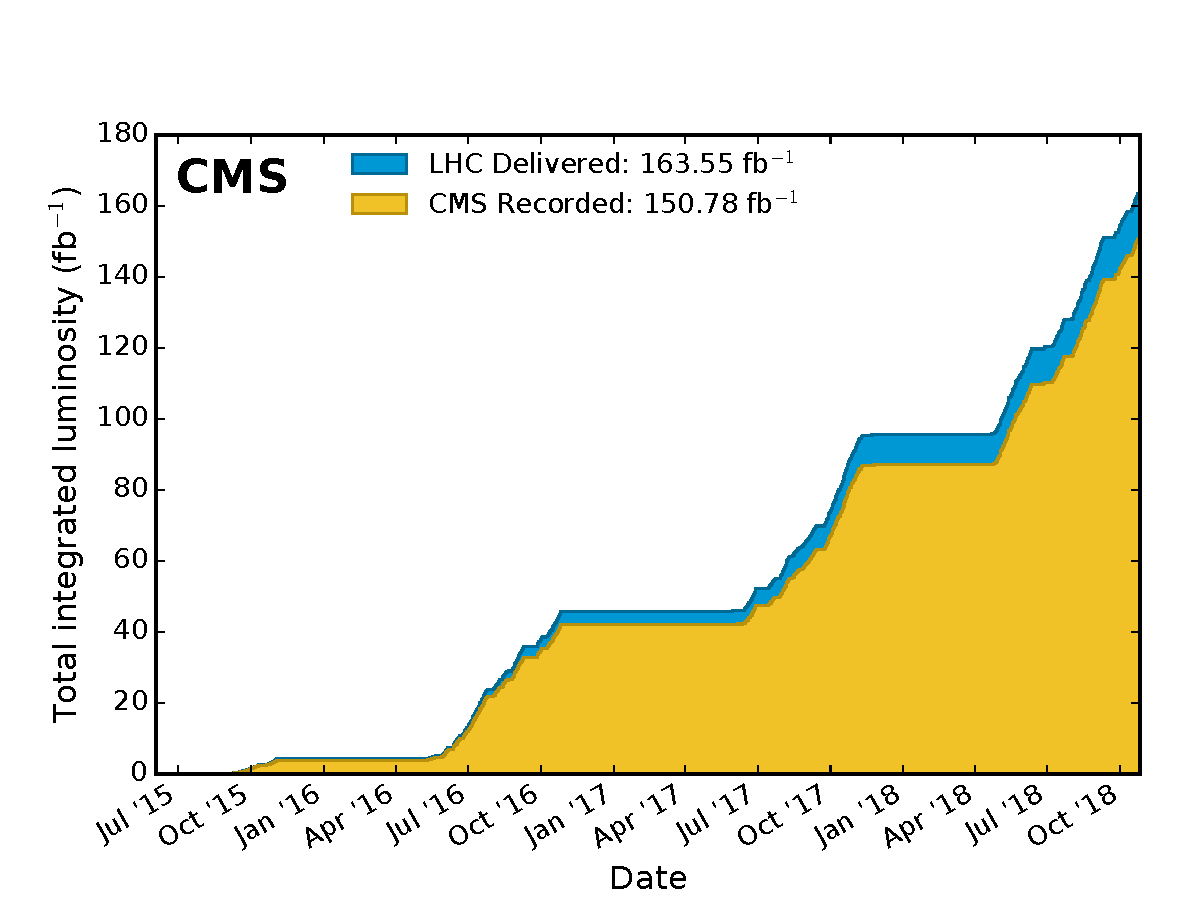
\includegraphics[width=0.7\textwidth]{Figures/Detector/LHC/lumi.pdf}
  \caption[Delivered and Recorded Luminosity at CMS, Cumulative Over 2015 to 2018]{Delivered and recorded luminosity at CMS, cumulative over 2015 to 2018. Figure taken from Ref.~\cite{LumiPubl64:online}.}\label{fig:lumi}
\end{figure}